\documentclass[a4paper,14pt]{scrartcl} 
\usepackage[utf8]{inputenc}
\usepackage[T1,T2A]{fontenc}
\usepackage[russian,english]{babel}
\usepackage{amsmath}
\usepackage{graphicx}
\usepackage{setspace}
\doublespacing
\usepackage{pdfpages}
\addto\captionsenglish{\renewcommand\contentsname{Оглавление}}


\begin{document}

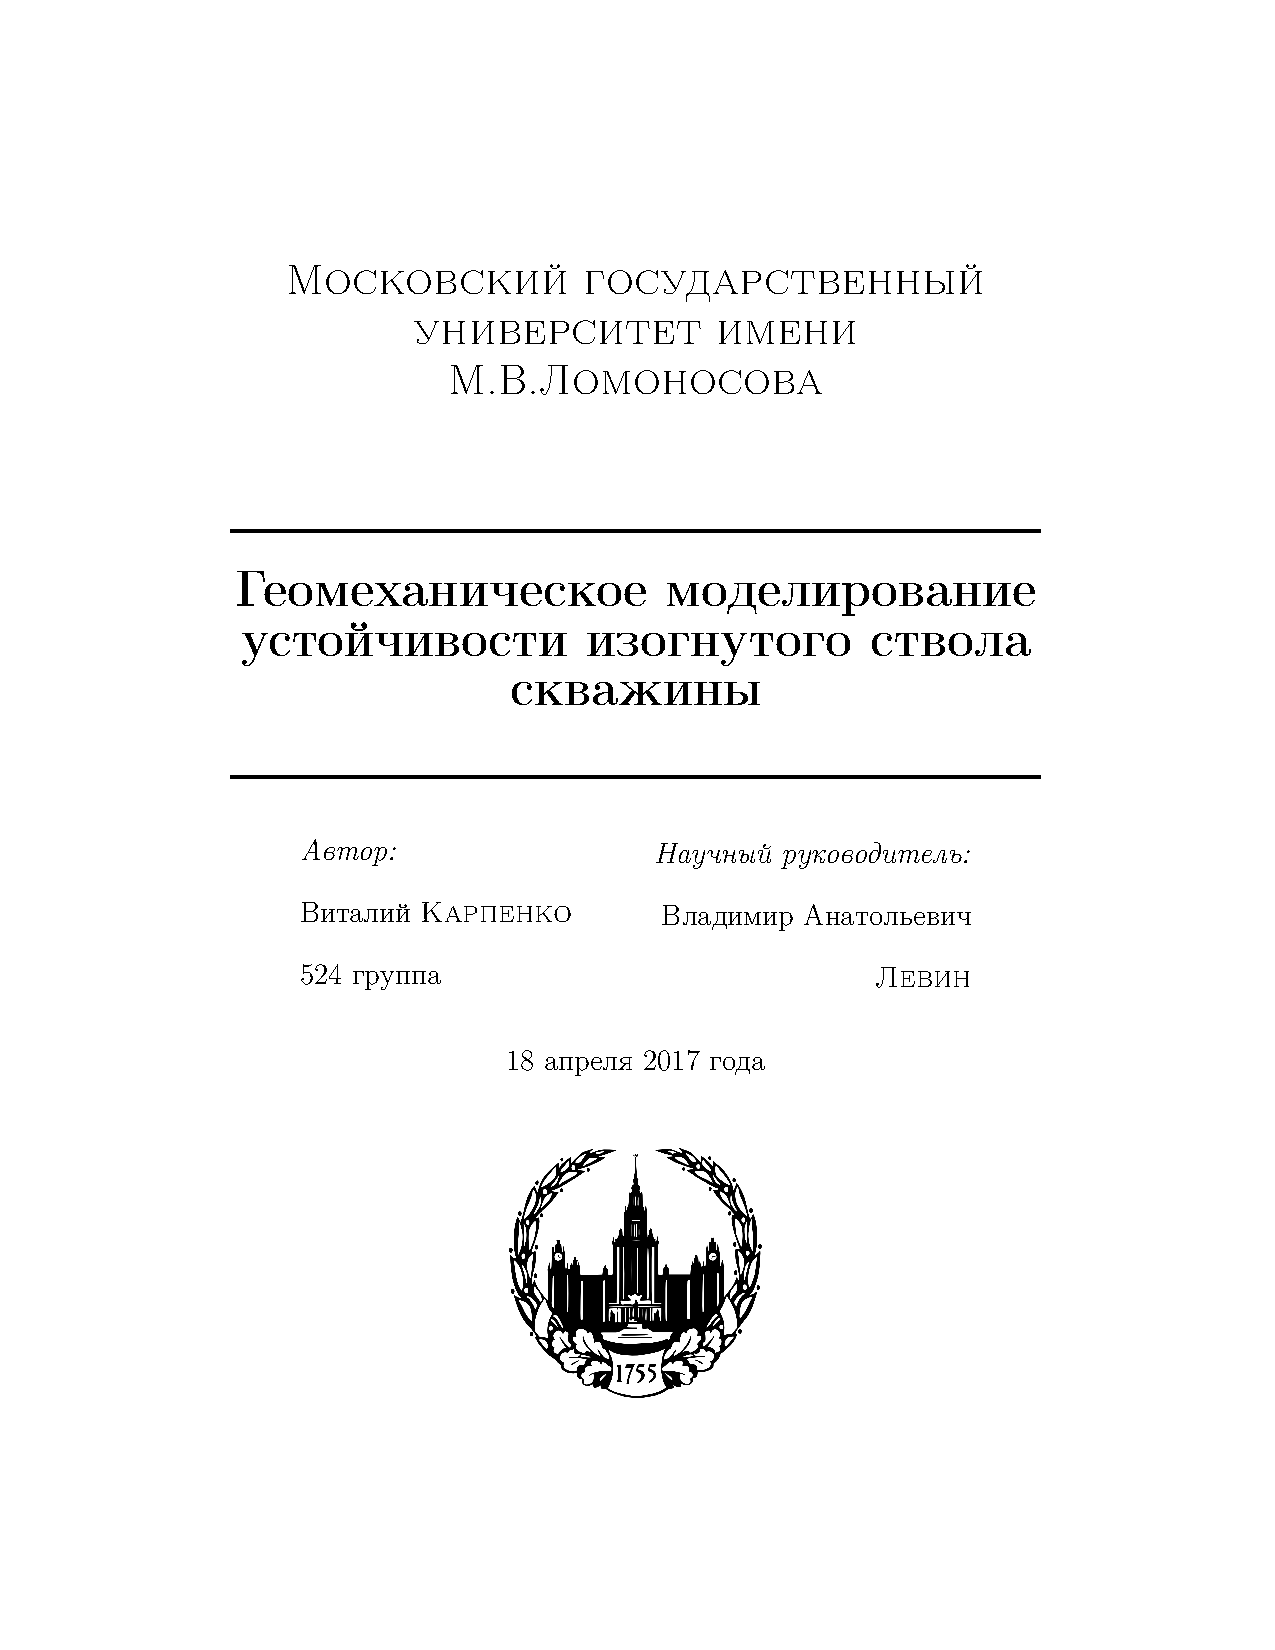
\includepdf[pages=1]{title.pdf}

\tableofcontents
\newpage

\section{Введение}
Определение технологических параметров, при которых ствол шахты будет сохранять стабильное состояние – одна из важнейших задач геомеханики.  

\end{document}
